
\documentclass[12pt]{article}
\usepackage[utf8]{inputenc}
\usepackage[english]{babel}
\usepackage{graphicx}
\usepackage[T1]{fontenc}    
\usepackage[document]{ragged2e}
\usepackage{booktabs}       
\usepackage{float}
\usepackage{tabularx}
\title{%
\textbf{CS685: DATA MINING\\
REPORT ON ASSIGNMENT 1\\}
\rule{\textwidth}{2pt}
}
\author{% 
Abhas Kumar-20111001\\
M.Tech CSE\\
}
\date{23 September 2020}

\begin{document}
\begin{figure}[t]
\centering

\includegraphics[scale=0.4]{IITK.png}
\end{figure}

\maketitle
\begin{abstract}
\begin{center}
This document reports the significant results obtained while working with COVID-19 data for the duration between 15 March 2020 and 5 September 2020 , presents analysis of these results and finally draws few conclusions based on the analysis.
\end{center} 
\end{abstract}
\textbf{RESULTS AND ANALYSIS}

\begin{enumerate}

    \item During 15 March to 5 September 2020, 10 most affected districts of our country just on the basis of total confirmed cases are \textbf{Pune, Delhi, Bangaluru Urban, Chennai,  Godavari, Kolkata, Kamrup, Ahmedabad,Lucknow,Patna} in decreasing order.
    
    And 10 least affected districts are \textbf{Aizawal, Dadra and Nagar Haveli, East Sikkim, Imphal, Solan, Papum Pare, Leh, East Khasi Hills, Dimapur, South Goa} in increasing order.


\pagebreak
\begin{figure}[H]
\centering
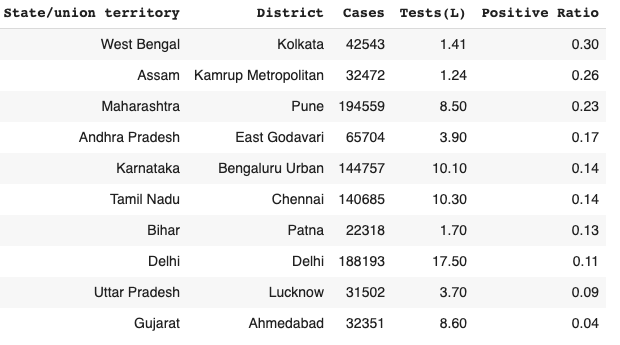
\includegraphics[scale=.6]{Test_ratio.png}
\caption{Showing Districts with test positive ratio in decreasing order}
\end{figure}

\item Whereas top 10 districts on the basis of test positive ratio ratio(confirmed cases/total tested) are \textbf{Kolkata, Kamrup, Pune, East Godavari, Bangaluru Urban, Chennai, Patna, Lucknow, Ahmedabad} in decreasing order (Figure 1).
    

\begin{figure}[H]
\Centering
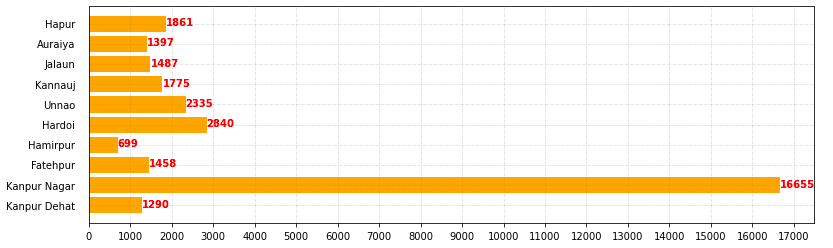
\includegraphics[scale=.6]{Kanpur_comp.png}
\caption{Kanpur with its Neighbor districts}
\end{figure}
\item Kanpur nagar alone had \textbf{16655} covid cases which was more than than all its neighbor district's cases combined, that was \textbf{15142}(Figure2).
\begin{table}[hbt!]
        \centering
        \small{
        \begin{tabular}{|c|c|c|c|}
        \hline
                Region & Number of States/UT & Total Cases & Average Cases\\
             \hline
                South India & 5 & 1332750 & 266550\\
             \hline
                 North India & 9 & 660664 & 73407 \\
             \hline
                West India & 5 & 1083601 & 216720  \\
             \hline
                East India & 5 & 484832 & 96966\\
            \hline
            Central India & 2 & 113549 & 56774 \\
            \hline
            Northeast India & 7 & 119562 & 17080 \\
             \hline
        \end{tabular}}
        \caption{Cases in Major 6 regions of our Country}
        \label{tab:dep}
    \end{table}\\
\begin{figure}[H]
\Centering
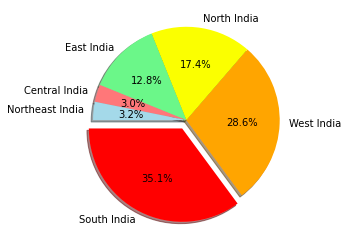
\includegraphics[scale=.6]{Pie.png}
\caption{Portion of total cases each of 6 regions had}
\end{figure}
 \end{enumerate}
 
\textbf{CONCLUSIONS}
\begin{enumerate}
    \item Ratio of Positives to tested is a better parameter than absolute number of confirmed cases for any region. Although \textbf{Pune} had most confirmed cases but it had only \textbf{23 positive cases out of 100} tested, whereas \textbf{Kolkata} had \textbf{30 positives per 100}.
    
    \item Southern and Western part of India are most affected regions.
    Southern and Western part with total of 10 states had \textbf{63.7\%} of total cases in India while rest 4 regions with 23 states had only \textbf{26.3\%} cases.
    
    \item Districts having metropolitan cities like \textbf{Delhi, Mumbai, Puna, Chennai, Bangaluru, Kolkata} are most affected regions which is in accordance with the fact that they have huge population and also large number of testing have been done in these major cities.
\end{enumerate}
\end{document}